\subsection{Bipolartransistor} % (fold)
\label{sub:Bipolartransistor}
\begin{frame}
    \frametitle{Bipolartransistor}
    \framesubtitle{Ziel}
    \begin{block}{Ziel:}
         \begin{itemize}
             \item Ausmessen der charakteristischen Daten des BC 548C
             Transistors
             \item Erstellen eines Vierquadrantenkennlinienfelds
         \end{itemize}
    \end{block}
\end{frame}
\begin{frame}
    \frametitle{Bipolartransistor}
    \framesubtitle{Schaltung}
    \begin{figure}[H]
    \begin{center}
            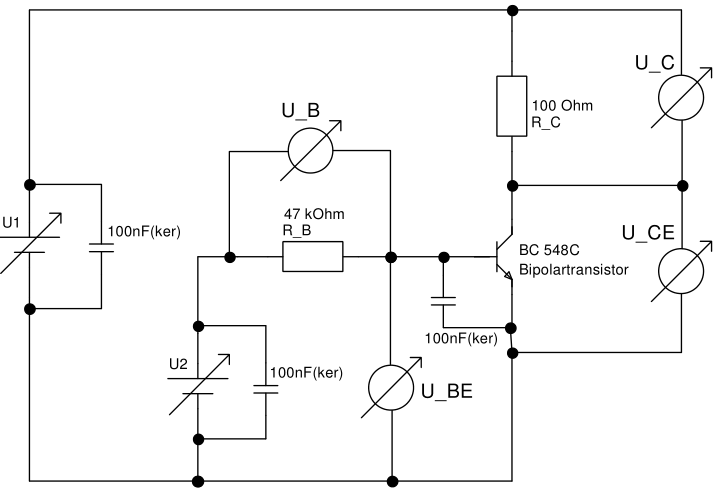
\includegraphics[scale=0.35]{./img/schaltungen/bipolarschaltung.png}
    \end{center}
    \end{figure}
\end{frame}

% subsection Bipolartransistor (end)
